%------------------------------------------------------------------------------
\chapter{Problems with segment selection algorithm for new triggers} 
\label{sec:app_3}
%------------------------------------------------------------------------------
\begin{figure}[h!]
\centering
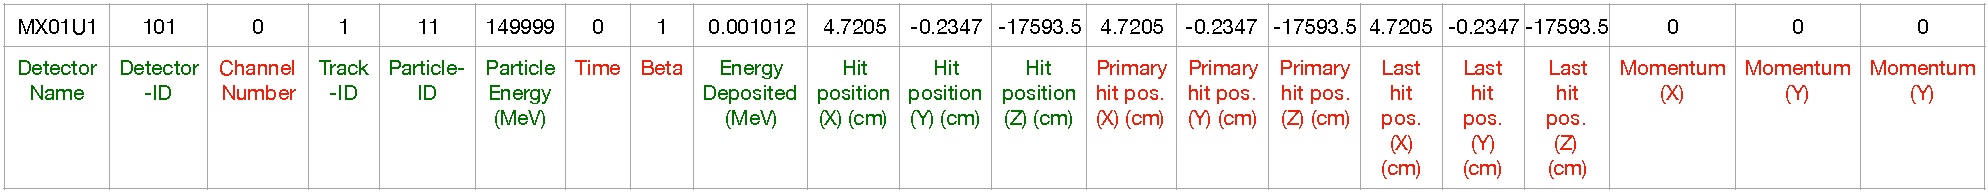
\includegraphics[width=18cm]{thesis_figures/TGEANT_format.pdf}
\caption{Snippet of the format fed to CORAL}
\label{fig:Format}
\end{figure}

This appendix aims to present some interesting reconstructed events that were observed in the background training sample when new triggers were used for the neutrino analysis. As mentioned before in sec.~\ref{} and described in more detail in~\cite{} a segment selection process is applied to improve the quality of angular reconstruction. A small example of the working of the process is shown in fig.~\ref{}. It was observed while performing the neutrino analysis with new triggers some events were mis-reconstructed due to an untuned segment selection algorithm. These events were further checked and reconstructed using the standard reconstruction used for inclined UHECRs at the Pierre Auger Observatory. It was also noticed that the problems with the segment selection algorithm for the new triggers could primarily arise from the presence of multiple peaks with similar amplitudes in the waveform. There is also an argument that the primary purpose of the segment selection algorithm i.e. the reduction of accidental muons which change the start time of the signal might already be addressed with the design of the new triggers thus decreasing the overall need for such an algorithm. However, these are only hypothesis and need to be confirmed with further studies. Thus, due to the inability to confirm the validity of the segment selection process for the new triggers, the algorithm was not applied to stations with these triggers in a way that the reconstruction for stations with old triggers remained unaffected. 